
\chapter{Method}

In order to evaluate how neuroevolution can be used to find racing behaviours a number of experiments will be conducted. The experiments require a controlled environment which can be reasoned about and where results can be reproduced. This chapter will cover the implementation of our experiment suite, which includes a racing simulator, an implementation of the NEAT-algorithm, a visualisation system and a control layer which connects the system components. Additionally, the reasoning behind and implementation of the experiments that were conducted will be presented. 

\section{Requirements of the simulator}
% What kind of behaviour do we want to find?
% Desired behaviour -> put requirements on the simulation
% Simulation -> desired behaviour is optimal

The purpose of this study is to evaluate how well a machine learning algorithm can manage to learn the key aspects of an effective racing behaviour. Some of the aspects that will be evaluated are positioning throughout corners, timing and speed management. 

If the behaviour of the AI is to be assessed in comparison to real world racing theory, the optimal behaviour in the simulated environment must be similar to the optimal behaviour in reality. The simulation may approximate certain aspects or neglect details, as long as the general characteristics remain and the best practises in racing theory are still optimal. % Lite knölig mening. 

This requirement on the simulation introduces some constraints to the physics simulation. For example, if positioning the car on the far side before taking a corner is to be optimal, the turning radius must increase with the speed of the car and accelerating or decelerating must be relatively slow. Taking a late apex before a straight will only be optimal if a larger initial speed onto a straight outperforms taking a smoother turn due to a slow acceleration rate. 

% Discuss negative effects of braking or accelerating while turning. 

\section{Implementation of the Simulator}
% Givet vårt beteende, hur evaluerar / analyserar vi saker i simulationen. Förklara vår sandlåda / universumet vi skapar.

The simulation is an iterative process where the state of the universe, which only consists of the car and the track, is updated continually. Each update represents a time interval of $10$ milliseconds within the universe. The updates are carried out in direct sequence, thus the simulation rate depends on the clock frequency of the computer running the simulation. However, with the speed of today's computers, a lot of simulation updates can be carried every second. This enables a modest desktop computer to simulate years of racing in a few hours. 

The car is represented by a simplified model of a car. Only the required properties discussed in the previous section are simulated. Each update of the car state results in an update of the cars position according to:

\begin{equation}
    \vec{p} = \vec{p} + \vec{v}\Delta t 
\end{equation}

Where $\vec{p}$ is the position vector of the car, $\vec{v}$ is the velocity vector of the car and $\Delta t$ is the delta time or the time-step, which is fixed at $0.01$ seconds.

The velocity vector $\vec{v}$ is updated due to acceleration based on the forces acting on the car. According to classical mechanics the acceleration $a$ of an object is equal to the applied force $f$ divided by the mass $m$ of the object, a relationship which is described by the equation $f = ma$. This can be extended into higher dimensions by representing the applied force and the acceleration as vectors with one value per axis. Thus the acceleration vector can be found with:

\begin{equation}
    \vec{a} = \frac{\vec{f}}{m}  
\end{equation}

All the forces that interact with the car are applied along the axis of the cars movement, i.e. no forces accelerating the car laterally are considered. Lateral movement, i.e. skidding, of the car is also excluded from the simulation. 

% FORMULA FOR TURNING RADIUS

The car weight used in the simulation is 642 kilogrammes, which albeit being oddly specific is a reasonable weight for a Formula 1 car without a driver. The rules state that the minimum weight of a car including the driver in full gear but excluding fuel is 702 kilogrammes \cite{f1_weight}.

The tracks used in the simulator are flat 3D-meshes with triangle faces. The meshes were modelled in Autodesk Maya and were imported as OBJ-files. In order to simplify the representation of the track the cross sections of the track are extracted from the mesh. These cross sections are treated as a series of checkpoints that define the track.  

It is assumed that the presented model fulfil the requirements presented in section 1, and that it does not introduce aspects that in any other way changes the characteristics of the optimal behaviour.

%section{Visualisation ???}

\section{NEAT Implementation}

The NEAT algorithm was implemented in C++ primarily based on the descriptions in the original paper \cite{stanley:neat}. Two implementations were also used as references, the latest C++ implementation from the authors themselves \cite{neat_source} and a script written in Lua used in a Super Mario bot \cite{mario_source}. 

In order to verify the implementation of the algorithm it was tested by training it to approximate the logical exclusive-OR function (XOR). The reason that the XOR-function is relevant to test is because it is not linearly separable, this means that a neural network requires hidden nodes in order to approximate it \cite{haykin:xor, stanley:neat}. The test was used as a sanity check to ensure that the algorithm made additions and changes to the network structure. 

% Ta upp skilnaden mellan NEAT och fs-NEAT?
Some minor utility features were added to our implementation in order to allow for a more flexible training process. For example, the activation function used in the neural networks is specified as a lambda-function, thus it can be changed at run-time. This enables us to specify what activation function should be used within a specific experiment. Furthermore, the ability to toggle the creation of an initial structure for new networks was added. If the option is enabled, the genomes start with a lattice of connections that connect each input to each output with a randomised weight. 


\section{Training Process}
% Hur går vi till väga för att träna en AI, hur är AI och träning kopplat till resten av systemet
% Hur ser träningen ut:
    % AIn styr bilen i varje simulation step
    % Indata, förklara inte vilken typ av indata, säg bara vart den kommer ifrån.
    % Slutgiltliga resultatet av simulationen ger feedback
The training process works by letting the neural networks adjust or train to drive the car. The combination of the NEAT algorithm and the simulator is utilised to perform training of the genomes. The actual learning, i.e. changes to the genomes, is the responsibility of NEAT. However, the evolutionary process requires a measurement of fitness to evaluate genomes. Thus the training procedure is responsible for calculating the fitness of every genome so that the evolutionary process can proceed. 

In order for the training process to evaluate a genome and calculate its fitness, the simulator is utilised. Calculating the fitness requires information about how well a specific has performed. The training process generates a network based on the genome that is to be evaluated, and feeds it to the simulator. The simulator uses this network to control the car during the simulation. In each update of the simulation, the simulator feeds data about the car and its environment into the network, with which the network calculates how to steer the car. Once the simulation terminates, the simulator presents the training process with a result that can be used to calculate the fitness.

The following subsections cover in detail the input and output to the networks supplied by and given to the simulator, as well as describing how genomes were evaluated and how fitness has been calculated to approximate network performance in an optimal way.

\subsection{Interpretation}
\label{method:interpretation}
% Talk about how the environment is represented in relation to the neural network.
% How does the AI see the world? What does the inputs look like?
% What kind of output does the AI give to steer and control the vehicle?
% NOTE: Explain the potential solutions, but do not give away which one is being used in the final version, this conclusion needs to come from performing experiments and should thus be presented in the discussion & results.
% Problem modelling. 
% used indata:
% bias
% distance to middle
% distance to left edge
% distance to right edge
% angle to track/mid line
% speed of car 
% corner data, points at [m]:
% 	10
% 	24
% 	42
% 	66
% 	100
% 	144
% 	205
% 	287
% 	397
% 	546
% sums of corner points:
% 	Segment 1, point 1-4, 10-66m
% 	Segment 2, point 4-7, 66-205m
% 	Segment 3, point 7-10, 205-546m

For the system to decide on some action for the car to take, it needs information about the car and its environment. Deciding on appropriate information to give to the system is an important aspect for NEAT to be able to progress in an efficient way. How effective any given input is, highly depends on the problem that is to be solved and what the target behaviour is.

The inputs used during the project aim to give an easy way for the system to couple situations with an appropriate action. The input values are summed up in table \ref{tab:input_table} and can be divided into two groups; One that describes the shape of the track in front of the car, and one that describes the current state of the car. Even though not all inputs were used in every experiment, they are all present in at least one experiment.

\begin{table}[h!] 
  \centering
  \begin{tabular}{ll}
    \toprule
    Name & Description\\
    \midrule
    Car speed & The current speed of the car\\
    Angle to mid line & Angle between the car direction and the track mid line\\
    Distance to middle & Distance between the car and the track mid line\\
    Distance to left edge & Distance between the car and the left edge of the track\\
    Distance to right edge & Distance between the car and the right edge of the track\\
    Track curvature & 10 angles describing the curvature of the track. \\
    Sums of curvature points & Three sums of track curvature angles 1-4, 4-7 and 7-10\\
    Bias & The value 1 to be used as a constant base value in neurons\\
    \bottomrule
  \end{tabular}
  \caption{List of all available neural network inputs.}
  \label{tab:input_table}
\end{table}

\noindent

There are two groups of input values describing the shape of the track in front of the car. These inputs aim towards letting the system plan ahead for the car, in order to adjust race lines before arriving at corners. 

The first group is the curvature data, which is a series of angles. The angles are based on the position of the car and 10 points on the mid line of the track. The first angle is calculated from the direction that the car faces and the direction to the first point. The rest of the angles are calculated by comparing the directions of the succeeding line segments the points stow. The distance between the points increase exponentially by 35 percent for each point. The points are distanced from the car by 10, 24, 42, 66, 100, 144, 205, 287, 397, 546 meters. The exponential increase of distances makes the resolution higher close to the car where detail is most important, and less resolution where the general tendency is sufficient.

The second group is three different summations of the curvature data, namely 1-4, 4-7 and 7-10. This will provide more of an overview perspective than the individual curvature points.

The set of inputs that describe the current status of the car are more simple in nature. They aim towards giving the system the capability of keeping the car on the track at all times. These inputs consist of current car speed measured in meters per second, angle between the cars current direction and the mid line of the track, distance from the car to the tracks mid line, as well as the distance between the car and the left and right edge of the track.

Additionally, a bias value is introduced as an input to the network. The value of this input will always be 1. This is due to the fact that if all inputs to a specific neuron are zero, the neuron would not be able to produce a signal. Since the output of a neuron is the weighted sum of all its inputs, the bias can be used to produce a base value for the sum. 

The number output values for the networks used during the project are limited to two. One for turning rate and one for acceleration and braking. The values for turning rate are in the range $[-1,1]$, where negative values represents steering right and positive ones to the left. If the output value of a network exceeds the amount of steering that can be applied at the current car speed, the simulator floors the value to that maximum. For the acceleration and breaking, the output values ranges from $[-1, 1]$, where positive values represents accelerating and negative values breaking. The value is interpreted by the simulator as a percentage of the cars current capability of accelerating and breaking.

% The turning rate value has the range $[-1,1]$, where negative values means steering to the right and positive to the left. If the value exceed how much the car turn at the current speed, the car will only turn as much as it can. The acceleration and braking value has the range $[-1, 1]$. Positive values mean that it should accelerate and negative values that it should brake. The value is a percentage of how much it it able to accelerate or brake.

% This subsection will define and motivate the different input and output configurations used in the experiments. Not all of them was used for every experiment, but this section serves to be referenced, in order to avoid redundant descriptions.

% Two different output values have been used in experiments, one for turning rate and one for acceleration and braking.

% The turning rate value has the range $[-1,1]$, where negative values means steering to the right and positive to the left. If the value exceed how much the car turn at the current speed, the car will only turn as much as it can.

% The acceleration and braking value has the range $[-1, 1]$. Positive values mean that it should accelerate and negative values that it should brake. The value is a percentage of how much it it able to accelerate or brake.

% When it comes to the different input values, the amount of different values are slightly larger.

% Some of the optional values describe the current state of the car. One of the them is the speed of the car, measured in meters per second. Then values are used for the distance to the middle of the track and the distances to the right and left edge of the track. Another value is the angle between the direction of the car and the mid line of the track.

% Another set of values describe the shape of the track ahead. One method used is consider the mid line of the track. It then picks points on that line with a fixed distance spacing, and takes the angles that separate the imaginary line segments between the point. In this way.

\subsection{Evaluation}
% Prata om fitness funktionen, men den behöver även "arbetas fram ur experimenten".. på något vis? Vi hade ju inte denna från början, den kom fram som en biprodukt av experimenten?
% Tänk också på läsaren, vad är lättast för den som läser att förstå
% Fitness functions

Running a simulation will give three values, the time the car was driving, the distance the car drove and how far the car came along the track. Worth noting is that the driven distance and the distance on the track is not necessarily the same, as the distance driven is affected if the car take curves on the inner and the outer side or drive in a serpentine.

How these three values are considered will effect what properties the neat will find. It is important to find a fitness function that not structurally encourage an unwanted behaviour.

The fitness function currently being used considers the distance along the track as well as the lap time. The fitness function is described mathematically by equation \ref{eq:fitness_distance_time}. It is important to note that the fitness will not be affected by the lap time unless the car actually performs a complete lap.

\begin{equation}
\label{eq:fitness_distance_time}
  f(d, t) =
  \begin{cases}
    d    & \quad \text{if } d < d_{max} \\
    d    & \quad \text{if } t \geq t_{max} \\
    d_{max} + 5*(\sqrt{t_{max}} - \sqrt{t})^2    &\quad \text{else} \\
  \end{cases}
\end{equation}

\noindent
This function aims to let the system train at one task at a time. The goal is that since lap time is not considered before a lap has been completed, the complexity of completing a lap will be reduced. When a lap has been completed, the goal is for the system to learn to optimise that lap by minimising the lap time. 
%[TODO: Add "It is interesting to see the difference between optimising for two variables after one another, instead of both at the same time"?]






\section{Experiments}

The project was an iterative process. Progress was made by experimentation, where different ways to model the problem and train the AI were tried out. In order to establish which aspects of the target behaviour that can be found with NEAT, a number of experiments of varying complexity were conducted. The following subsections will motivate the need for the different experiments and explain how they were conducted. 

\subsection{Steering a car moving at a constant speed}
\label{method:constant_speed}
Driving a car is a complex problem, consisting of several sub-problems. This experiment aims to reduce the problem to one of its components, the steering. Instead of learning to control every aspect of the car, the AI will learn to steer a car that travels forward at a constant speed. The speed is sufficiently low to allow the car to take every corner on the circuit. 

%% TODO infoga bild på banan?

Two variations of this experiment were conducted with different car speeds. In the first variant, the system learns to steer but is only given local perception of the environment, which in this case means that the car knows its position and orientation relative to the road. In the second variant the number of inputs is increased and the car is given the curve data. Thus the car receives information about the shape of the track ahead.

These experiments will give insight into how well the AI can interpret the provided data and how an increased perception of the track shape affect the behaviour. The AI successfully learning to steer the car would ensure that such behaviours can be found with NEAT and show which of the provided pieces of information that are relevant to solving the problem. If the AI learns to steer only using a subset of the inputs, it shows that the other information is not required in order to steer

% TODO: Formulera om: Without any curvature information, the AI is unable to plan ahead.
% Det känns som en slutsats, det borde kännas mer som det är logiskt sjävklart.
Comparing the result of the different experiment variants should show whether or not the addition of curve data will enable the AI to plan ahead and how that affects the behaviour of the AI. Without any curvature information, the AI is unable to plan ahead. Since it is only aware of the current position and orientation of the car, it is only able to react to that information. It seems reasonable that providing information describing the shape of the track ahead of the car will enable the car to plan ahead. Thus improving the AI's ability to take difficult corners and steer effectively. 

% Stuff that could be included in the text above:
% 1. It should also help with deciding whether or not the way in which the track and steering actions are represented needs to be modified in any way, in order to increase network performance.
% 2. When gradually incrementing the speed, what kind of race line do we want the car to perform?

% BAKA IN
%In order to allow the network to plan ahead, a set of new inputs to the network was introduced. The concept of curve data, as explained in section 3.4.1 was provided to the network. Initially, the distance ahead covered by the new input data was 100 meters, but it was later expanded to 300 meters and 500 meters. Other than this change in input data, the inputs and outputs of the network were the same as in the fixed speed experiment.

% Examining this will present relevant information regarding what to expect once the complexity of the problem is increased. It should also help with deciding whether or not the way in which the track and steering actions are represented needs to be modified in any way, in order to increase network performance.

% TODO: Rewrite this once Training Process -> Interpretation has been written, so that we can refer back to that section. 
%The input data to the neural network in this experiment consists of the angle between the car and the mid line, curve data and the sum of the curve data absolute values as well as the current distance from the car to the mid line. The output that is produced by the network is an evenly distributed float value that ranges from $-1$ to $1$, representing full steering to the right and left respectively.

%In order to further increase the complexity of the problem and to examine the possibility of the AI to calculate an optimal race line, the aspect of planning ahead was introduced. The constant speed of the car was increased to a level were going around certain corners in the middle of the track, would not be possible. Thus forcing the network to position the car on a race line that has a larger radius than driving in the middle of the track. Performing this experiment should give some insight into the capabilities of the AI with regards to modifying race lines in order to take a complete lap. Even though the AI might not be able to take the most optimal route, seeing the capabilities of the race line modification could present some interesting information about potential problems or modifications needed.


\subsection{Full control of the car}
\label{method:baseline}
In this experiment, the AI will train on driving with full control of the car. In addition to steering it will also control the speed by accelerating and braking. In addition to the position, orientation, and curvature data the AI will be provided with the current speed of the car. The result of the experiment will further establish the limits of the training system. 

Several experiment variations with this configuration will be carried out. In the first variant, which is the baseline experiment, the AI will drive on the same complete circuit as used in the constant speed experiments. This will show whether or not the AI is able to stay on the track to the same extent as when it only steers. Furthermore, it will show whether or not the system can learn to manage the speed in an effective way. If the system is able to find an effective behaviour, the natural response would be to even further increase the complexity of the problem. However, if no effective behaviour is found, it is and implication that the training process and system configuration are suboptimal. 

\subsection{Short Track Segments}
\label{subsec:shorttracksegment}
This variant of the experiment will test the system on shorter track segments, only containing one corner each. The motivation for testing short tracks is that it should be easier for the system to find effective behaviours on a short segment than on a complete circuit. This is because the behaviour required to complete a long circuit is generally more complex than the behaviour needed to complete just one corner. Thus the algorithm will be able to start optimising for speed earlier and on less developed genomes. 

The tracks consist of two straights connected by a corner. The straights are between $400$ and $500$ metres long and there are three types of corners used. The first corner is a $30$ degree corner that the car should be able to drive quite fast through. The second one is a $90$ degree corner with a small inner radius. The third corner used is a hairpin corner which turns $180$ degrees with a small inner radius. 
\begin{figure}[H]
    \centering
    \subfloat[The 30 degree corner.]{{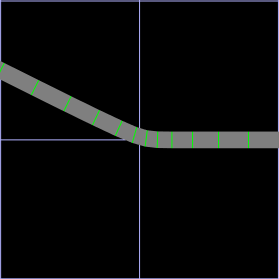
\includegraphics[width=0.28\textwidth]{corner_30}}}%
    \qquad
    \subfloat[The tight 90 degree corner.]{{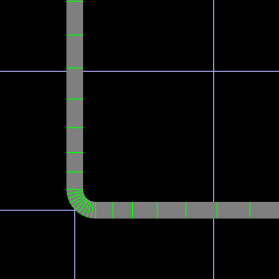
\includegraphics[width=0.28\textwidth]{corner_90}}}%
    \qquad
    \subfloat[The 180 degree hairpin corner.]{{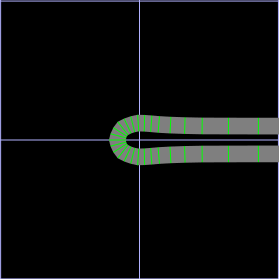
\includegraphics[width=0.28\textwidth]{corner_180}}}%

    \caption{Aerial view of the three corner types. The Gray line is the track which is 12 metres wide.}
\end{figure}
Successful results in these experiments would confirm that the system can find effective behaviours for shorter track segments. If that is the case the training process for the short track segments could be extended to solve more complex problems. A scenario where the experiment yield significantly more effective behaviours than the baseline experiment would give insight into the limits of the training process and how the fitness function is used. This insight could be used to find effective behaviours for longer tracks. 

%==================================================================
\subsection{Multiple short track segments}

If the system finds effective behaviours on the short track segments, one interesting experiment is to train the same population on multiple short segments. Finding behaviours effective at several different types of corners is one step towards a generally effective behaviour. Training on multiple track segments could be a safer training environment for the genomes because the consequences of failing on one segment is not necessarily catastrophic. A change that increase the effectiveness over one segment but leads to a crash on another would be catastrophic on the circuit. However, if the genomes are evaluated on several track segment, failures on one segment can be compensated for by performing well on others. 

The track segments used are the same ones as in the short track segment experiment with the addition of the mirrored versions of those segments. Thus the fitness of a genome is evaluated by summing the fitness acquired on each of the six tracks.

This experiment could answer two interesting questions. Is the system able to find behaviours effective in multiple scenarios and how do it differ to training different corners in a sequence in a single track? Additionally, how general would that behaviour be? Answers to these questions could give insight into how large the set of training scenarios required to find a fully general behaviour is. 
%====================================================================

%% SKRIV OM ALTERNATING TRACKS IFALL VI SKALL DET
%It will also be tested to alternate which of the track segments are used for the evaluation. Will this let networks progress further, since a temporary decline in some curves will not be noticed? 

\subsection{Mirrored Track}
\label{method:mirror}
One of the project goals is to find generalised knowledge of how to drive in the racing domain. This means that a genome learns to drive regardless of what track it drives on, instead of learning how to complete a specific circuit. In order to test this a population of genomes is trained on driving on the full circuit used in previous experiments. After a while some genomes will have learnt to complete the circuit. That population is then loaded into the same experiment except with another track which is a mirrored version of the one used earlier. This means that the genomes will drive on a track where each corner on the circuit has the same shape but opposite direction of the ones on the other circuit. The development of this population can then be compared to the development of a control group that is only trained on the mirrored track. 

%% TODO: Lägg in bilder där man kan se skillnaden på banorna med startposition och riktning utmarkerat så att man fattar.

There is a wide range of possible results in this experiment, in the worst case, the performance of the trained group is equal or worse than the control group and in the best case it performs as well as before the change of circuit. The best case scenario is unlikely, since the genomes will encounter corners they haven't encountered before. However, if the test population outperforms the control group in any significant way it shows that the population has acquired some general knowledge of how to turn or manage the speed. 

If the results show some form of generalisation there is a possible extension to the experiment that could yield interesting results. The extension regards the extent to which the population forgets knowledge about the original circuit when migrated. If the population is migrated back to the original track after learning how to drive on the mirrored one, will it still remember how to drive on it? Can the population learn to drive well on one track without forgetting how to drive well on the other?


